%% DOCUMENT SET UP
\documentclass{article}
\usepackage[top=1.0in, bottom=1.0in, left=1.0in, right=1.0in]{geometry}
\usepackage{graphicx}
\usepackage{float}
\usepackage{setspace}
\usepackage{mdwlist}
\doublespacing
\begin{document}
% title page
\begin{titlepage}
\begin{center}
% giant white space

\includegraphics{white}
% logo

\includegraphics[width=0.5\textwidth]{logo} \\ [3.5cm]
% text stuff
Annabel Hung \\
Dr. Zoe Wood \\
June 7, 2011
\end{center}
\end{titlepage}
\setcounter{tocdepth}{2}
\thispagestyle{empty}
\tableofcontents
\newpage
\thispagestyle{empty}
\listoffigures
\newpage
\setcounter{page}{1}

%% CONTENT

\section{Introduction}

Video gaming has become a major part of entertainment. In the past few years, its popularity has been increased by mainstream games such as Call of Duty, Halo, and World of Warcraft, along with smaller independent games like Super Meat Boy and Minecraft. Gaming is also one of the driving forces of computing technology, with complex games utilizing the power of new graphics and processor technology. Smaller and simpler games often expand the genre with an interesting artistic vision or simple gameplay. A subset of games, often labelled ``casual''
games, are simple easy-to-play games that appeal to a wide variety of gamers.
Because complex games are difficult to develop and require a lot of resources,
we decided that a casual game would be within the scope of our game development.
Thus we designed and developed a casual 3D video game for our senior project.

\subsection{Course Structure}

The course took place over two quarters, or roughly twenty three weeks. In the
first quarter, we focused on game pitches, the basic game concept, setting up
the programming environments, and programming the basic game system. We formed a
team of three people in the first few weeks of the first quarter. Our team
consisted of Christopher Gilson, Eric Fong, and myself. We programmed many aspects
of our game without art assets, and used simple spheres and simple art in order
to set up the game logic and basic gameplay. At the end of the first quarter, we
had a basic game with simple gameplay and simple art.

For the second quarter, Christopher Gilson left our team and took \textit{Food Fight} 
in a different direction. Eric and I continued work on our game, adding a
few new features, fixing bugs and adding aesthetic changes into our game, and
adding additional art. After playtests, where other people played our game, we
altered the difficulty and asked them for their feedback, eventually
incorporating it into the final project.

\section{Project Overview}

\subsection{General Description}

\textit{Food Fight} is a casual arcade-style action game, where you control a kid and
throw food at other kids. The setting is in a modern cafeteria, and the
characters move around, throwing food at each other and eventually making the
cafeteria messier as the gameplay progresses. The goal of the game is to hit the
other kids with food in order to score more points in a limited amount of time. The other kids also throw food at you, so
avoiding them and avoiding the food they throw is key to getting a higher score.

The look and feel of the game is cartoony and cute. The characters are
exaggerated for aesthetic effect, and the proportions of food are unrealistic in
order to emphasize certain aspects of the game. Food splats are bigger than they
should be in reality, in order to give the player the sense of making the
cafeteria messy. The other kids have exaggerated bodies so that it is easier to
see where they are and hit them with food.

Because our game is a simple arcade-style action game, it does not have a long
story like other games. The game is, at its core, about a kid throwing food at
other kids, creating a mess of the cafeteria in the process. When different
people with different playstyles play the game, they may create different
stories when they play. For instance, one player may carefully throw food in
order to keep the cafeteria clean and only hit the enemy players, saving food
for scoring more points. Another player may not mind getting the cafeteria dirty
and wasting food, ensuring that they hit the other kids at the expense of extra
points.

\subsection{Technical Description}

We programmed our game using primarily C++ and OpenGL. C++ is a powerful
programming language that is widely used in the gaming industry. Because C++ is
similar to C, it was easy to work with and we were able to program in it easily
since all of our team members were familiar with it. C++ also has some aspects,
like classes and inheritance, that make it well suited to game development.
Certain objects in the game world can be classified and sub-classified using
inheritance, making game programming easier. For example, in our game, we
declare an entity object, representing both the player and the enemies. Our
collision logic works when comparing any two entities, and does not need to
worry about colliding the myriad of different types of entities present.
 
OpenGL is a cross-platform graphics library API that makes developing 2D and 3D
games easier. Our actual implementation of OpenGL has many parts, including
OpenGL (GL)\cite{gl}, OpenGL Utility (GLU), the free OpenGL Utility
Toolkit (freeglut/GLUT)\cite{freeglut}, the OpenGL Extension Wrangler
(GLEW)\cite{glew}, and the OpenGL Shader Language (GLSL)\cite{glsl}. The OpenGL
suite, consisting of GL, GLU, and GLUT, are what we used to draw and display all of the graphics to the screen. We used GLEW to
determine what functionality the graphics card in the machine possessed, and
then enable additional graphics functions to make them available to us. We
programmed additional graphics shaders in the GLSL, and enabled
graphics-approprate features (as reported by GLEW).

Another important technology we used in our program is Lua scripting.\cite{lua}
Lua is a lightweight programming language that is very well suited for scripting
events, information, and game actions into our game. We use Lua scripting to
create and process various game content, calculate updated values rapidly, and
load in user defined values at the start of the game. The flexibility of the
language and the program hooks are what allow us to add new content rapidly and
easily into the game.

\section{Related Works}

\subsection{League of Legends}

League of Legends is a strategy game developed by Riot Games, where
you control a single character and move them around a wide-open
battlefield, attacking other player characters and other units
controlled by the computer player. \cite{rofl} We looked at this game for several
things, primarily the control scheme and viewing angle. League of Legends has a
similar camera angle to our game, along with a similar style of gameplay. For
that reason, we modelled our game controls after theirs, using a simplified
version of their movement and attacking controls in our own game. League of
Legends also uses Lua to store, modify, and alter game values during gameplay.
We sought to emulate this model on a simpler scale.

\subsection{Fat Princess}

Fat Princess is a game developed by Titan Studios for the {PlayStation
3}.\cite{fat} This game had an art aesthetic similar to our game, along with a
similar camera angle. One of the things we used was the music from Fat Princess;
we felt that the style of the music matched our game, and the game had a comical
mischevious feel to it, two aspects that we wanted to emulate in our game. The
gameplay was also slightly similar to our game, in that you control one
character and attack other characters. However, because Fat Princess was only
available on the {PlayStation 3} at the time of our game development, we did not
look at it for control styles. The art style was very cartoonish, with lots of
solid primary colors and colors that made the game look cel-shaded.

\section{Algorithms}

\subsection{Overview}
The developers were allowed to exercise their creativity with the project, but they were also required to implement certain technologies in their project. Here is a list of all of the technologies included in \textit{Food Fight} as well as the name(s) of developers who had contributed to that technology. Following the list is a detailed description of my major contributions to the project.

\begin{itemize*}
    \item 3D Interactive Game Environment (Christopher Gilson, Annabel Hung, Eric Fong)
    \item Original Art and Models (Christopher Gilson)
    \item Audio and Sound Effects (Eric Fong)
    \item Lua Scripting (Eric Fong)
    \item Occupancy Grid (Annabel Hung)
    \item Collision Detection (Annabel Hung)
    \item Enemy Artificial Intelligence (Annabel Hung)
    \item View Frustum Culling (Christopher Gilson, Eric Fong)
    \item Particle System (Christopher Gilson)
    \item Game UI Overlay (Christopher Gilson)
    \item Food Selection System (Annabel Hung)
    \item Game State System (Annabel Hung, Eric Fong)
    \item Game Controls (Eric Fong)
    \item Collision and Game Logic (Annabel Hung, Eric Fong)
    \item OpenGL Shaders (Christopher Gilson)
    \item Shadows (Eric Fong)
\end{itemize*}

\subsection{Collision Detection}

\subsubsection{Description}
Collision detection is a very important part of \textit{Food Fight} because colliding objects together is central to the game. Without a properly working system, the project would not be successful. \textit{Food Fight's} collision detection system uses uniform spatial subdivision to divide the environment into equally sized volumes. Because most objects remain on the xz-plane, a two-dimensional rather than three-dimensional occupancy grid is used. 

Each volume maintains a list of the objects that are contained or partially contained in it. If the list ever contains more than one object, the objects in the list are checked against each other for collisions. If a collision has occurred, each colliding object reacts depending on what it has collided with. The following table summarizes the collision responses for each object (collision behavior for enemies are described in detail in Section 4.5.1): \\

\begin{figure}[H]
    \begin{tabular}{| l | l | l | l | l | l |}
    \hline
    \multicolumn{2}{|c|}{Player} & 
    \multicolumn{2}{|c|}{Food} & 
    \multicolumn{2}{|c|}{Obstacle} \\
    \hline
    Target & Response & Target & Response & Target & Response \\ \hline
    Enemy & Stop moving & Enemy & Player's? +1 score; remove & Enemy & Do nothing \\ \hline
    Food & Enemy's? Lose point & Food & Do nothing & Food & Do nothing \\ \hline
    Obstacle & Stop moving & Obstacle & Remove & Obstacle & Do nothing \\ \hline
    Player & Do nothing & Player & Remove & Player & Do nothing \\
    \hline
    \end{tabular}
    \caption{Object collision behavior.}
\end{figure}

\subsubsection{Implementation}
A \verb+boxel+ class has been created to represent the volumes that the environment is divided into. This class keeps its coordinates so it keeps track of the area that it covers. This class also uses a \verb+vector+ to keep track of the objects it contains. To determine whether an object is contained within the boxel, the object's bounding box (described below) is compared with the boxel's coordinates. In other words, using the boxel's coordinates to represent its ``bounding box,'' a collision check is performed between the boxel and the object. If a ``collision'' has occurred, then the object is contained in the boxel.

Every object in the game has a bounding box, defined when the models are loaded at the beginning of the game. During loading, the smallest and largest values for the x, y, and z vertices are recorded. These values are used to create the bounding box for the model. As each object keeps track of its own model, it also keeps track of its own bounding box with six variables for the minimum and maximum x, y, and z coordinates.

\begin{figure}[H]
  \centering
    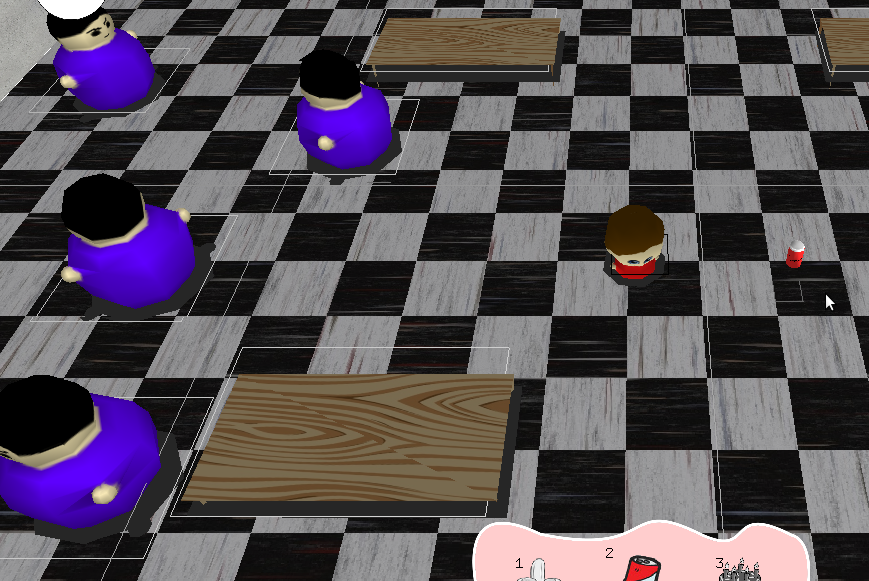
\includegraphics[width=0.7\textwidth]{boxes}
    \caption{The occupancy grid and bounding boxes are shown in white.}
\end{figure}

To determine if a collision has occurred between two objects \verb+objectA+ and \verb+objectB+, a check to see if the bounding boxes are overlapping is performed. This check is done by seeing whether \verb+objectA+'s minimum x is greater than \verb+objectB+'s minimum x but less than \verb+objectB+'s maximum x. The other dimensions are checked as well. The logic for this check is found in the \verb+collides(objectA, objectB)+ function, which uses \verb+if+ statements to compare x, y, and z coordinates for overlap.

If a collision between two objects has occurred, then each object's \verb+collide(target)+ is called with the collided object as its argument. Though the logic for each object is different, the structure of this function is the same. A series of \verb+if+ statements matches \verb+target+'s type with the appropriate response.

\subsection{Game State System}
Published games often have features in addition to the actual playable portion, such as an options menu. In order to make \textit{Food Fight} more complete in terms of these features, a game state system was developed. Such a system also makes maintaining the structure of the application as a whole easier. \textit{Food Fight} has four distinct states: \verb+MAIN_MENU, FOOD_SELECTION, PLAYING, SCORE_SCREEN.+ Each state corresponds to certain sections of the game that are different from the others because it provides the player with different information, goals, and choices. Different events can occur depending on the current state of the game.

\subsubsection{Description}
If the current state is \verb+MAIN_MENU+, the player is presented with the game's menu. From here, the player can see the game's logo and pick between playing the game or terminating the application. If the player clicks the button labeled ``Play,'' the game state changes to \verb+FOOD_SELECTION+. If ``Quit'' is chosen, then the application closes. \verb+FOOD_SELECTION+ is the only state that this state can change to.

\begin{figure}[H]
  \centering
    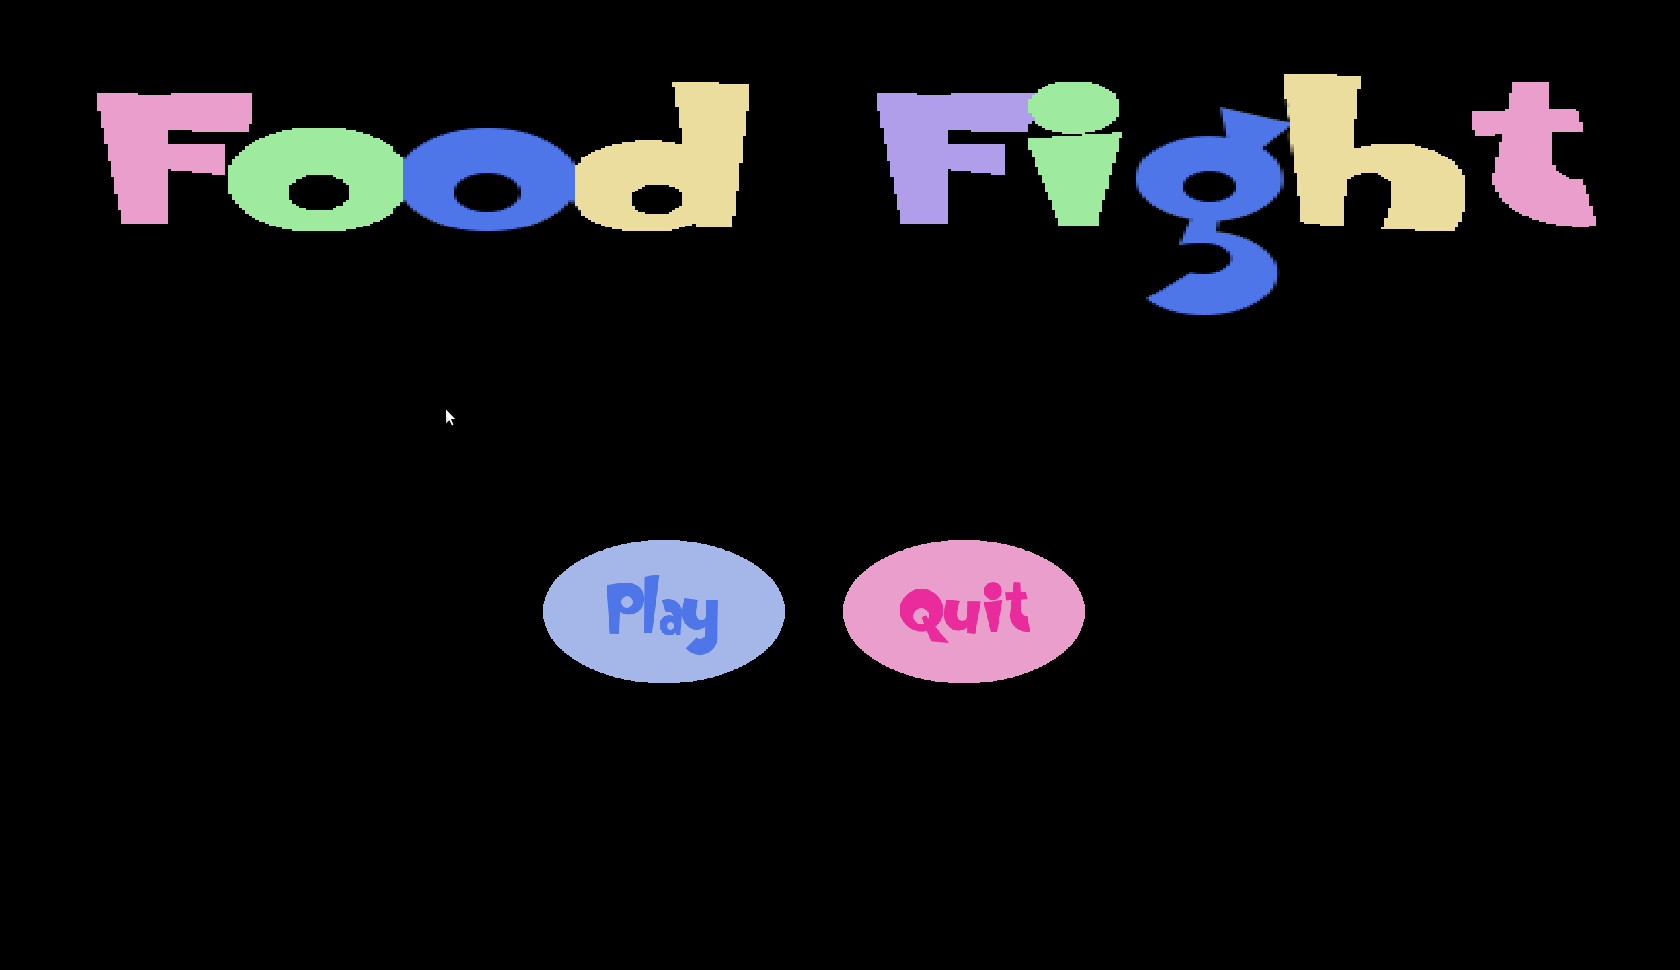
\includegraphics[width=0.7\textwidth]{mainmenu}
    \caption{Main menu screen in Food Fight.} 
\end{figure}

As the name of this game state suggests, \verb+FOOD_SELECTION+ is where the player is presented with the different types of foods and their prices, and can select which he or she would like to use during the game. The food selection system is described in detail in Section 4.4. From this state, the player can click ``Ready'' to progress to the \verb+PLAYING+ state.

\verb+PLAYING+ is the state for the actual playable portion of the game. During this state, the player can see the cafeteria environment, populated with enemies and obstacles as well as the player's own model. The player is able to interact with the environment using left mouse clicks to throw food and right mouse clicks to move. Keyboard keys 1, 2, and 3 allow the player to select the food that they would like to use next. A counter also keeps track of score. This state differs from the other states in that it is the only state that is timed, lasting one minute. Once the timer reaches zero, the state automatically changes. This state will also change if the quantity for all three of the player's foods ever reaches zero. The only state that this state can change to is \verb+SCORE_SCREEN+.

The \verb+SCORE_SCREEN+ state is similar to \verb+MAIN_MENU+ in that it displays a bit of information and provides only two actions for the player to choose from. The score from the round of game play that just ended is displayed, and the player can choose to either play another round or go back to the main menu. Clicking on ``Retry'' will change the state to \verb+PLAYING+. The player will be using the same foods from the previous round. Clicking on ``Menu'' will change the state to \verb+MAIN_MENU+. If the player wishes to play again using different foods, he or she will have to start from \verb+MAIN_MENU+ in order to access the food selection screen. The \verb+SCORE_SCREEN+ state differs from the other states in that there are two states (as opposed to one) that it can change to.

\begin{figure}[H]
  \centering
    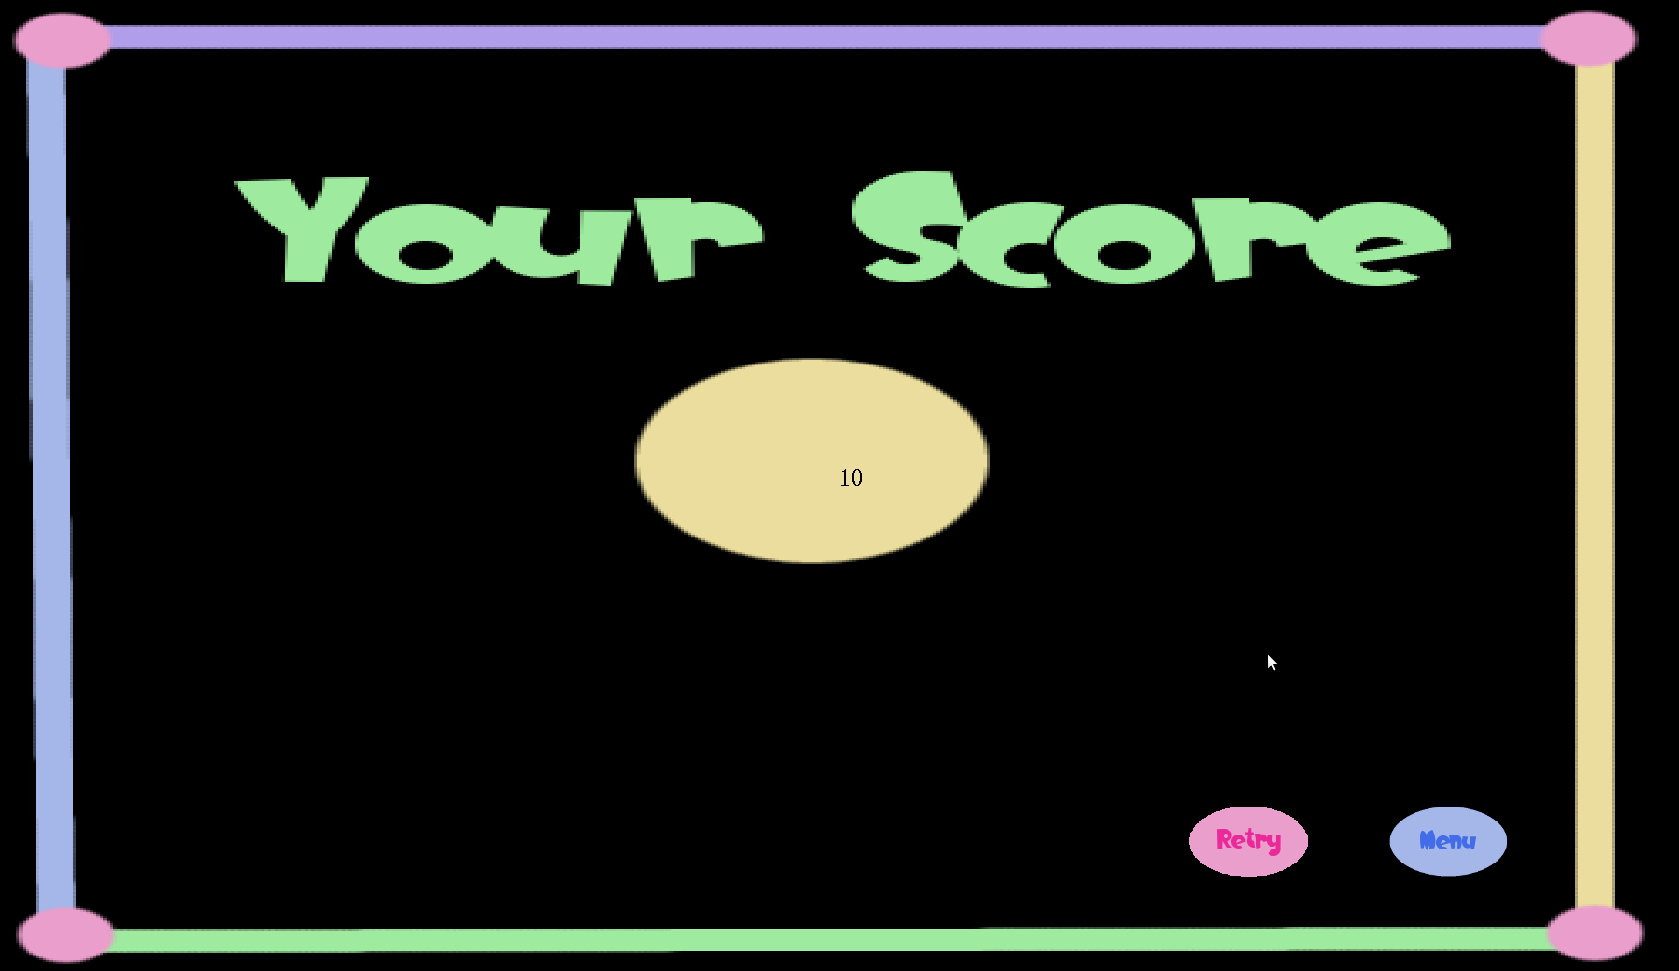
\includegraphics[width=0.7\textwidth]{scorescreen}
    \caption{The score screen in Food Fight.}    
\end{figure}

\subsubsection{Implementation}
The implementation of the game state system is fairly simple. The states are represented with an \verb+enum+, and a single \verb+currentState+ variable keeps track of the current game state. To change the state, a special function \verb+changeState(newState)+ is called to handle the transition, where \verb+state+ is the desired state to change to. This function prevents incorrect state changes by checking the current state with the \verb+newState+. The function also handles any overhead work, such as resetting the score and timer counters when restarting a game. \verb+if+ statements are used in various parts of the code to determine what objects to display or what logic to use. For example, when the current game state is \verb+MAIN_MENU+, there is no need to display the current score or the enemies. The game state system helps ensure that computations are only made when they are necessary.

The following diagram sums of the flow of control for the game state system:

\begin{figure}[H]
    \centering
    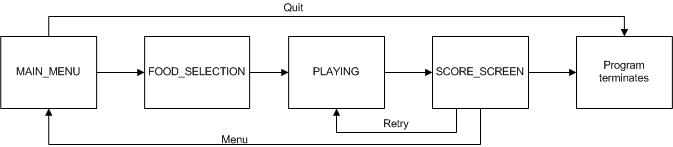
\includegraphics{gamestate}
    \caption{Diagram of the game state system.}
\end{figure}

\subsection{Food Selection System}
Even though the current version of \textit{Food Fight} has foods that only differ in appearance, the system to allow for the player to select which foods to use during game play is completely implemented. The purpose of this system is to ease the transition between selecting foods and playing the game. The foods were implemented in a generic fashion such that this system will work with any future new foods. The following is a description of how this system works.

\subsubsection{Description}
Before the player begins playing and scoring points, he or she must first select which foods to use. Each of the foods is displayed with its price and quantity. The amount of money that the player can spend on food is also shown. Each food picture acts as a button that the player can click to select that food. Clicking on a food button will add that food item to the food bar displayed on the bottom of the screen and deduct the corresponding amount of money from the user's allowance. A reset button is provided in case the player changes his or her mind about the current selection. Clicking this button will clear the foor bar and return the money back to the player. 

\begin{figure}[H]
  \centering
    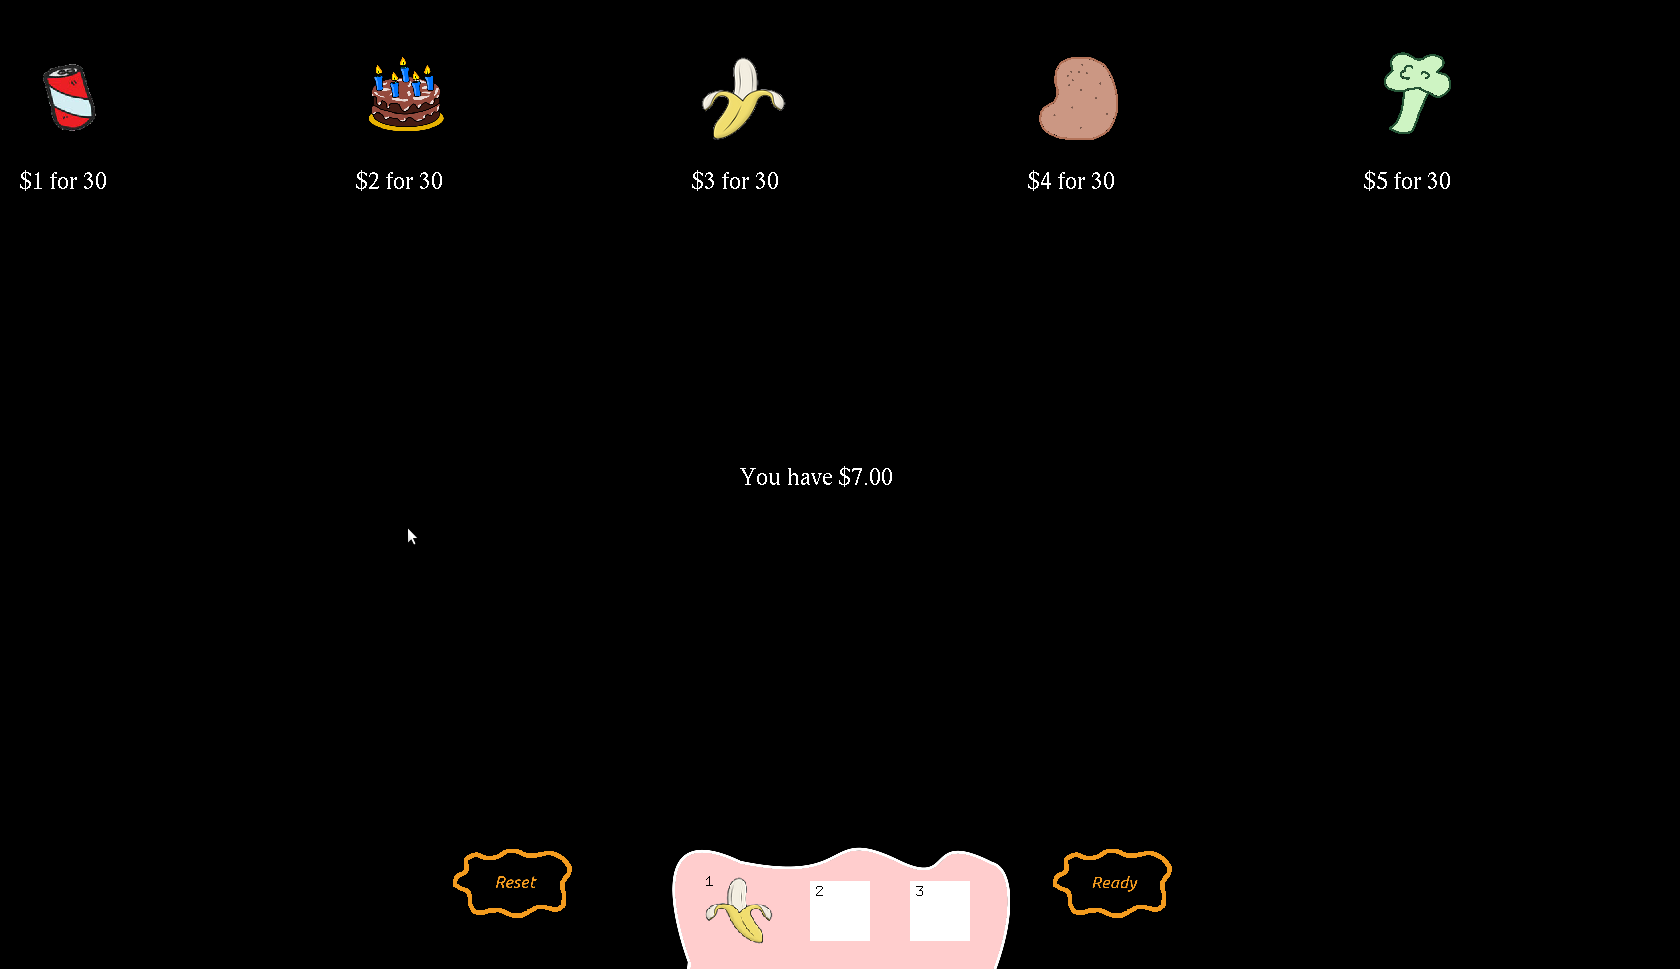
\includegraphics[width=0.7\textwidth]{foodselect}
      \caption{The food selection screen in Food Fight.}
\end{figure}

There are two restrictions placed on the player in this part of the game. First, the player may not spend more than their allotted amount of money. Though in the current version the only difference between the foods is the model, this limitation will encourage the player to spend their money wisely once foods with different effects are implemented. Secondly, the player must select exactly three foods. This decision was partially for ease of implementation, but also to encourage the use of more foods. Because the player needs to throw food at enemies in order to score, having more food will give the player more chances to earn points, so the player would actually put themselves at a \textit{disadvantage} if they do not give themselves as much ammunition as possible.

\subsubsection{Implementation}
The ``buttons'' that are used in this system are created by binding textures to rectangles placed on the display screen. The coordinates and sizes of these rectangles are used by the OpenGL \verb+mouse()+ callback to check whether the coordinates of mouse clicks are within the areas covered by the rectangles. If the mouse coordinates overlap with the rectangle's area, then the button is considered clicked.

Much of the logic for this system is also found in the \verb+mouse()+ function. Each food is assigned a number, and variables \verb+first, second,+ and \verb+third+ keep track of which foods are selected. These variables also help prevent the player from selecting the same food more than once. Another variable is used to keep track of the amount of money remaining, which also helps prevent the player from purchasing food that he or she cannot afford. Lastly, when the "Ready" button is clicked, \verb+first, second,+ and \verb+third+ are checked for valid values before the player can begin playing. This ensures that three foods have actually been selected.

\subsection{Artificial Intelligence}
In order to provide a challenge for the player, the enemies are given very simple intelligence. This intelligence is in the form of a set of rules defining the enemy's behavior. The enemies in \textit{Food Fight} are best described as simple reflex agents because they will perform an action if the conditions for that action are met. The following is an in-depth description of the enemy's behavior as well as implementation details.

\subsubsection{Description}
If the enemy is moving around and collides with another object, a number of events can occur. Depending on the type and state, and sometimes the owner, of the collided object, the enemy will react in a certain way. For example, if an enemy collides with food thrown by the player, its corresponding action is to fall down. The following table shows the various conditions for collisions that can trigger an action: \\

\begin{figure}[H]
    \centering
    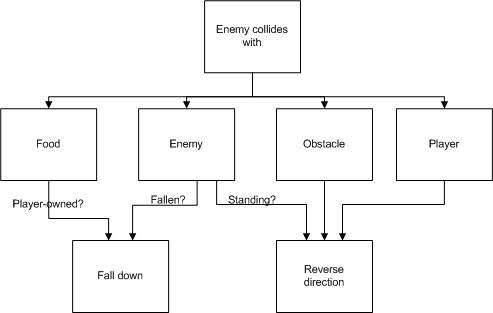
\includegraphics{enemyAI}
    \caption{Diagram of enemy collision behavior.}
\end{figure}

The enemy also responds to a few other events that do not involve collisions. These include attacking the player and internal timers.

If the enemy is moving around and detects that the player has come within a certain distance, it has the opportunity to throw food at the player. However, whether or not the enemy can actually attack the player depends on its internal timer. After an attack, the enemy must wait three seconds before it can attack again. It is important to note that the enemies have knowledge of the player's position at all time. However, this knowledge is not used for anything beyond calculating the distance to the player.
 
As noted in the table above, if the enemy is hit by food thrown by the player, it must fall down. In this state, the enemy cannot take any actions until another internal timer has finished counting down. Once the timer is up, the enemy can change its state back to standing and continue moving around.

\subsubsection{Implementation}
The enemy's logic is split into two functions in the \verb+enemy+ class. Part of the logic can be found in its \verb+collide()+ function, which takes the collided object as an argument. This function's structure is a series of \verb+if+ statements that considers the type of collided object and then executes the code for the appropriate response.

The other part of the logic is in the \verb+update()+ function. The timers are maintained by this function. Also, the code for checking whether or not the player is nearby is in this function. This is done by using the enemy's position and the player's position with the distance formula. If the distance is less than or equal to a certain value, then the enemy will attack if its attack timer allows it. The distance that is considered within range has been adjusted according to feedback from playtesters, as described in Section 4.

\section{Results}

\subsection{Accomplishments}
Despite missing enhancing features, \textit{Food Fight} has progressed from a simple idea to an actual game. The first step was to ensure the application functioned properly, and then to find a balance between the game's difficulty and entertainment value.

We believe that we have developed a game that is fun and challenging with a good level of replayability. Perhaps the best feature about \textit{Food Fight} is that many players have found it quite amusing to throw food and make a mess while trying to earn points. Because our game has very simple rules and controls, a new player would not need to deal with a steep learning curve and can immediately begin enjoying the game. We also feel that the art and music selection both compliment the game, adding to its cute and funny style. Overall, we are most proud of creating a playable game that people can actually enjoy.

\subsection{Images}
Here are some additional screenshots of our game.

\begin{figure}[H]
  \centering
    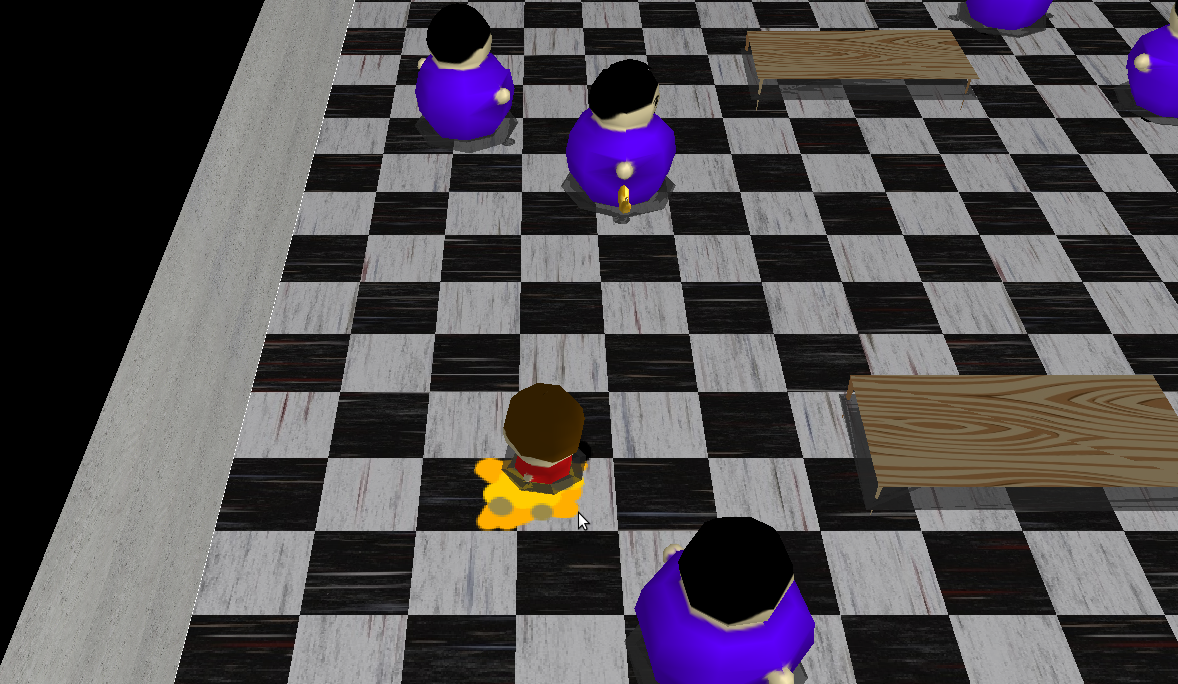
\includegraphics[width=0.7\textwidth]{enemiesattacking}
    \caption{Enemies attacking the player.}    
\end{figure}

\begin{figure}[H]
  \centering
    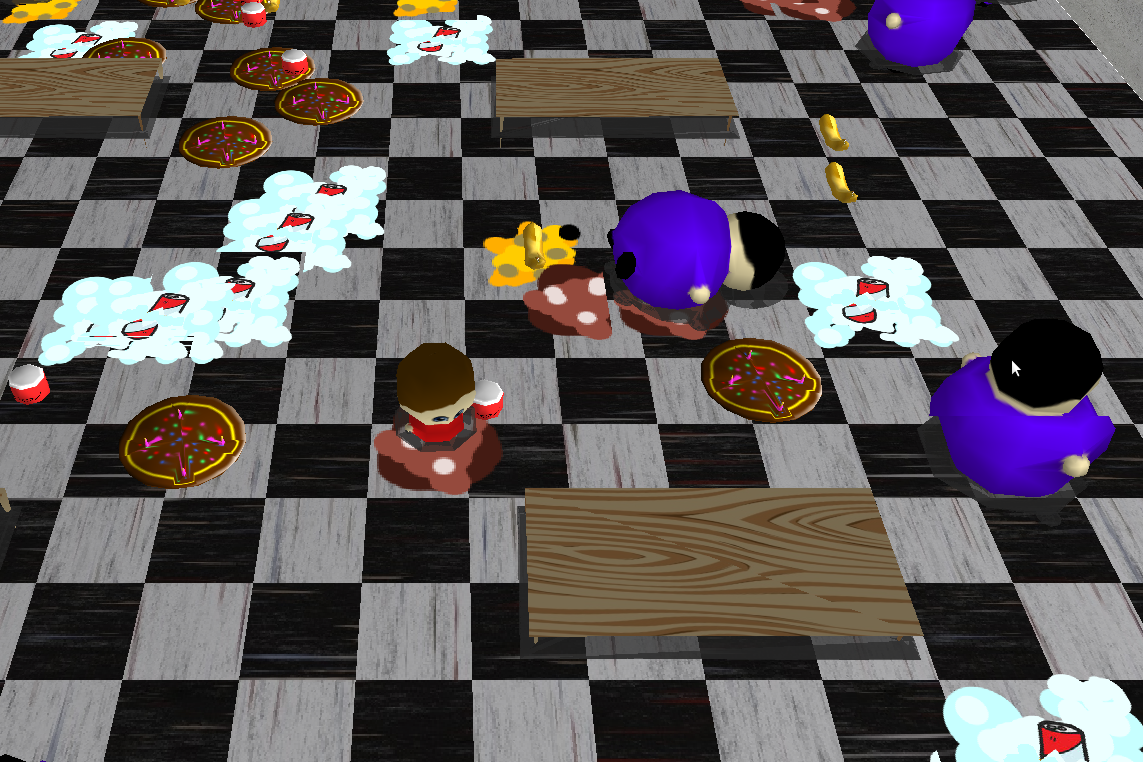
\includegraphics[width=0.7\textwidth]{enemiesfallen}
    \caption{Enemies fallen down after hitting food.}    
\end{figure}

\begin{figure}[H]
  \centering
    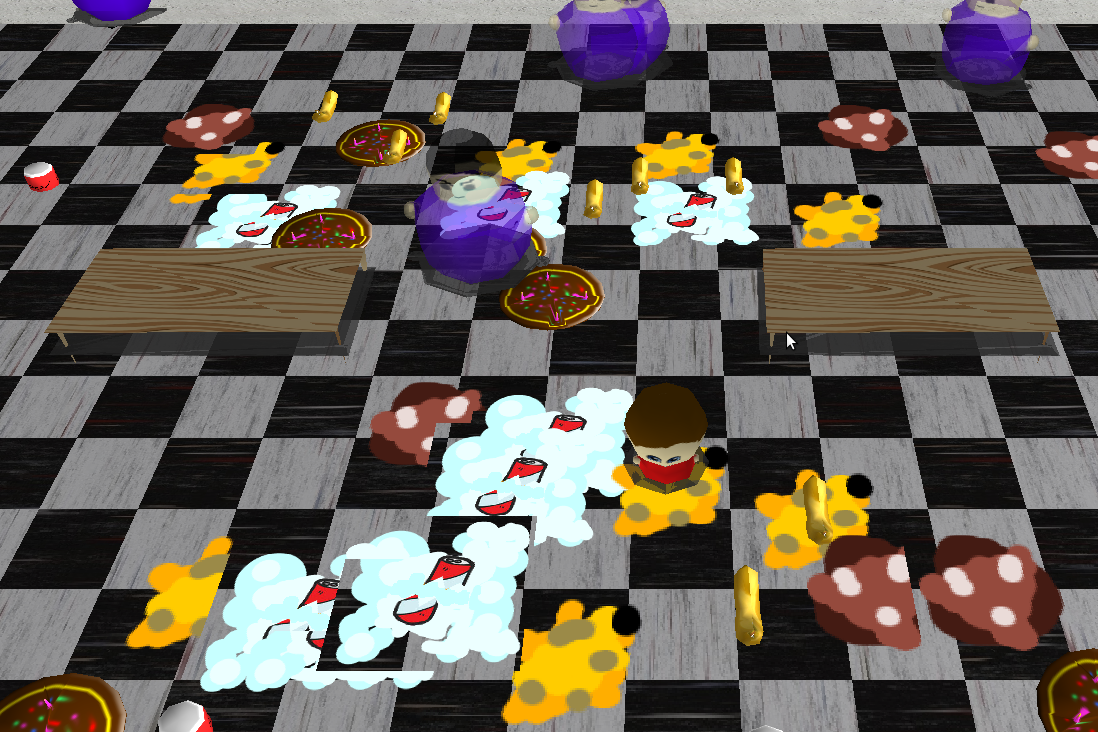
\includegraphics[width=0.7\textwidth]{enemiesinactive}
    \caption{Enemies are slightly faded for a few seconds after getting up.}    
\end{figure}

\subsection{Player Feedback}
Throughout the development process, several people have tested the game and provided feedback. Many of the complaints were related to the game's difficulty, so a good portion of development time was spent adjusting the difficulty so that it was still challenging but not excessively so. The following is a summary of what some people have said about the game after playing it: \\

\begin{figure}[H]
    \begin{tabular}{|p{1cm}|p{2cm}|p{3cm}|p{3cm}|p{5cm}|}
    \hline
    Tester & Stability & Fun & Difficulty & Suggestions \\ \hline
    1 & 5 of 5 & 4.5 of 5 & too hard with many enemies & temporary invincibility after getting hit \\ \hline
    2 & No crashes & Cute, funny idea & Really hard, controls are weird & Make it easier \\ \hline
    3 & stable & Sort of fun & Hard, too easy to keep getting hit & Make the enemies not throw so much \\ \hline
    4 & stable & Pretty fun, funny idea & Controls fine; AI is hard at first & Differentiate foods \\ \hline
    5 & good & Cute & Hard controls, game is too hard & Make enemies attack less \\
    \hline
    \end{tabular} \\
    \caption{Summary of player feedback.}
\end{figure}    

The game has been adjusted to lower the difficulty in the following ways:
\begin{itemize}
  \item The player will no longer fall down when hit. Players were frequently hit and thus spent most of the game time unable to run away.
  \item The amount of time the enemy between enemy attacks has been increased.
  \item The distance considered within range between an enemy and the player has been increased.
\end{itemize}

However, to keep the game from becoming too easy, the difficulty has been increased in the following ways:
\begin{itemize}
  \item An enemy is worth no points while he is fallen.
  \item An enemy is worth no points for a few seconds after getting back up.
\end{itemize}

\subsection{Development Process}
Because our team consisted of only three (and then reduced to two) members, we did not really have a team manager. For both quarters, the project was divided into two parts, graphical and logical. Because we had to begin writing code soon after our idea was approved, there was little time for planning, such as project design and work assignments. As a result, the team ended up with code that was difficult to maintain and an imbalanced work distribution.

The end of the first half of development saw changes, both good and bad. The good effect was a massive code reorganization, which made the second half of development significantly easier. The bad effect was the loss of the team member who was most experienced with graphics. The team dealt with this reduction by focusing on improving the gameplay portion of the game, which was their strength. Their hope was that even though the game did not look as well as it may have, it would still be a very fun game to play.

\section{Conclusion}
Personally, this project was an enormous learning experience. Because my specialization for this project was collision detection, I am now very familiar with this technology. I also gained experience as a game developer, especially learning to adjust the game appropriately after receiving feedback.

As a programmer, I also gained more experience following good coding practices, such as writing maintainable code and using version control. Prior to this project, I had not used Git for version control but can now add it to my list of tools. I also learned the value of planning on paper prior to coding: it was easier to understand (and thus implement) the food selection and game state systems after drawing out diagrams of their structure.

I also learned the value of communication when working in teams. With a team size of two, during the second half of development we always worked on the project together. It was very helpful to be able to quickly ask each other questions or discuss ideas or problems. However, because we only dealt with each other, it was really important to be polite and courteous. My teammate and I had a close relationship prior to the project and still do because we were able to realize that 

\section{Future Work}
The following are some of the features for this project that unfortunately were not implemented in the current version. The main reason for excluding these features was the focus on perfecting more critical aspects of the project. For example, it was more important to implement the enemy than to implement different types of enemies. However, because the project was designed with expansion in mind, different enemies can be easily supported once their artificial intelligence is developed. Likewise, the other features would not be difficult to add.

\subsection{Different Foods}
Because the game is about having a food fight, having a wide variety of foods to choose from would add to the appeal of the game. As mentioned before, the only difference between the foods is their appearance, or their model. It would be more challenging if foods can have different effects on the enemies, such as slowing enemy movement or hitting multiple enemies at once.

Another idea involved foods that the player could consume for temporary bonuses. Examples include an increase in movement speed or a shield to block enemy attacks.

If different foods were implemented, the game play would change significantly because more strategic planning would be required on the player's part. The player would be able to select foods that are better suited to their playstyle, or try to find a good combination of foods to maximize their score. Differentiating the foods would make their role in the game more meaninful and the overall game more fun.

\subsection{Different Enemies}
In the current version, there is only one type of enemy with simple behavior. Different enemies would also change the game play significantly because it would change the difficulty of the game. This would allow more players to enjoy the game: new players can select to play with easier enemies while experienced players can test their skill against more challenging enemies.

Besides different behavior, different enemies would be worth different amounts of points. This would add some strategy to the game in that the player would have to think about which enemies are worth attacking. For example, there could be an enemy worth many points that won't attack the player, but is surrounded by several aggressive enemies that are worth few points. The player would have to decide how best to approach this group of enemies.

\subsection{High Score List}
Implementing a high score list would add to the arcade feel of the game. After all, the goal of the game is to earn as many points as possible. In the current version, the score is not very meaningful as it is lost once a round of play is over. If scores were recorded and viewable as a list, players could compare their scores with their peers, which would invite friendly competition. There would actually be a reason to try to earn as many points as possible.

%% DOCUMENT WRAP UP

\newpage
\bibliographystyle{IEEEannot}
\bibliography{document}
\end{document}
